%package list
\documentclass{article}
\usepackage[top=3cm, bottom=3cm, outer=3cm, inner=3cm]{geometry}
\usepackage{multicol}
\usepackage{graphicx}
\usepackage{url}
\usepackage{hyperref}
\usepackage{array}
\newcolumntype{x}[1]{>{\centering\arraybackslash\hspace{0pt}}p{#1}}
\usepackage{natbib}
\usepackage{pdfpages}
\usepackage{multirow}
\usepackage[normalem]{ulem}
\useunder{\uline}{\ul}{}
\usepackage{svg}
\usepackage{xcolor}
\usepackage{listings}
\lstdefinestyle{ascii-tree}{
    literate={├}{|}1 {─}{--}1 {└}{+}1 
  }
\lstset{basicstyle=\ttfamily,
  showstringspaces=false,
  commentstyle=\color{red},
  keywordstyle=\color{blue}
}
%\usepackage{booktabs}
\usepackage{caption}
\usepackage{subcaption}
\usepackage{float}
\usepackage{array}

% Comment
\usepackage{verbatim}

\newcolumntype{M}[1]{>{\centering\arraybackslash}m{#1}}
\newcolumntype{N}{@{}m{0pt}@{}}


%%%%%%%%%%%%%%%%%%%%%%%%%%%%%%%%%%%%%%%%%%%%%%%%%%%%%%%%%%%%%%%%%%%%%%%%%%%%
%%%%%%%%%%%%%%%%%%%%%%%%%%%%%%%%%%%%%%%%%%%%%%%%%%%%%%%%%%%%%%%%%%%%%%%%%%%%
\newcommand{\itemEmail}{rzapata@unsa.edu.pe}
\newcommand{\itemStudent}{Reyser Julio Zapata Butron}
\newcommand{\itemCourse}{Análisis Y Diseño de Algoritmos}
\newcommand{\itemCourseCode}{1702231}
\newcommand{\itemSemester}{IV}
\newcommand{\itemUniversity}{Universidad Nacional de San Agustín de Arequipa}
\newcommand{\itemFaculty}{Facultad de Ingeniería de Producción y Servicios}
\newcommand{\itemDepartment}{Departamento Académico de Ingeniería de Sistemas e Informática}
\newcommand{\itemSchool}{Escuela Profesional de Ingeniería de Sistemas}
\newcommand{\itemAcademic}{2024 - B}
\newcommand{\itemInput}{19 noviembre 2024}
\newcommand{\itemOutput}{25 noviembre 2024}
\newcommand{\itemPracticeNumber}{06}
\newcommand{\itemTheme}{Estruturas de dados para grafos: Listas de adyacencia}
\newcommand{\itemPracticeDuration}{02 horas}
%%%%%%%%%%%%%%%%%%%%%%%%%%%%%%%%%%%%%%%%%%%%%%%%%%%%%%%%%%%%%%%%%%%%%%%%%%%%
%%%%%%%%%%%%%%%%%%%%%%%%%%%%%%%%%%%%%%%%%%%%%%%%%%%%%%%%%%%%%%%%%%%%%%%%%%%%

\usepackage[english,spanish]{babel}
\usepackage[utf8]{inputenc}
\AtBeginDocument{\selectlanguage{spanish}}
\renewcommand{\figurename}{Figura}
\renewcommand{\refname}{Referencias}
\renewcommand{\tablename}{Tabla} %esto no funciona cuando se usa babel
\AtBeginDocument{%
	\renewcommand\tablename{Tabla}
}

\usepackage{fancyhdr}
\pagestyle{fancy}
\fancyhf{}
\setlength{\headheight}{30pt}
\renewcommand{\headrulewidth}{1pt}
\renewcommand{\footrulewidth}{1pt}
\fancyhead[L]{\raisebox{-0.2\height}{
\includegraphics[width=3cm]{img/logo_episunsa.png}}}
\fancyhead[C]{\fontsize{7}{7}\selectfont	\itemUniversity \\ \itemFaculty \\ \itemDepartment \\ \itemSchool \\ \textbf{\itemCourse}}
\fancyhead[R]{\raisebox{-0.2\height}{
\includegraphics[width=1.2cm]{img/logo_abet}}}
\fancyfoot[L]{Reyser Julio Zapata Butrón}
\fancyfoot[C]{\itemCourse}
\fancyfoot[R]{Página \thepage}

% Estilos del Código
\usepackage{listings}
\usepackage{color, colortbl}
\definecolor{dkgreen}{rgb}{0,0.6,0}
\definecolor{gray}{rgb}{0.5,0.5,0.5}
\definecolor{codebackground}{rgb}{89, 0.97, 0.90}
\definecolor{tablebackground}{rgb}{0.8, 0, 0}

\lstset{
  language=C++,                  
  basicstyle=\ttfamily\footnotesize,
  keywordstyle=\color{blue},     
  commentstyle=\color{dkgreen},    
  stringstyle=\color{red},       
  backgroundcolor= \color{codebackground},
  numbers=left,                  
  numberstyle=\tiny\color{gray},
  stepnumber=1,                  
  numbersep=5pt,                
  showspaces=false,              
  showstringspaces=false,      
  showtabs=false,                
  frame=single,                  
  captionpos=b,                  %
}

\begin{document}
	\vspace*{10px}
	
	\begin{center}	
		\fontsize{17}{17} \textbf{ Informe de Laboratorio \itemPracticeNumber}
	\end{center}

 %% TABLA %%
 
	\centerline{\textbf{\Large Tema: \itemTheme}}

	\begin{flushright}
		\begin{tabular}{|M{2.5cm}|N|}
			\hline 
			\rowcolor{tablebackground}
			\color{white} \textbf{Nota}  \\
			\hline 
			     \\[30pt]
			\hline 			
		\end{tabular}
	\end{flushright}	

	\begin{table}[H]
		\begin{tabular}{|x{4.7cm}|x{4.8cm}|x{4.8cm}|}
			\hline 
			\rowcolor{tablebackground}
			\color{white} \textbf{Estudiante} & \color{white}\textbf{Escuela}  & \color{white}\textbf{Asignatura}   \\
			\hline 
			{\itemStudent \par \itemEmail} & \itemSchool & {\itemCourse \par Semestre: \itemSemester \par Código: \itemCourseCode}     \\
			\hline 			
		\end{tabular}
	\end{table}		
	
	\begin{table}[H]
		\begin{tabular}{|x{4.7cm}|x{4.8cm}|x{4.8cm}|}
			\hline 
			\rowcolor{tablebackground}
			\color{white}\textbf{Laboratorio} & \color{white}\textbf{Tema}  & \color{white}\textbf{Duración}   \\
			\hline 
			\itemPracticeNumber & \itemTheme & \itemPracticeDuration   \\
			\hline 
		\end{tabular}
	\end{table}
	
	\begin{table}[H]
		\begin{tabular}{|x{4.7cm}|x{4.8cm}|x{4.8cm}|}
			\hline 
			\rowcolor{tablebackground}
			\color{white}\textbf{Semestre académico} & \color{white}\textbf{Fecha de inicio}  & \color{white}\textbf{Fecha de entrega}   \\
			\hline 
			\itemAcademic & \itemInput &  \itemOutput  \\
			\hline 
		\end{tabular}
	\end{table}

 %% CONTENIDO %%
\section{Código base}
    El siguiente código presentado, es la base para la realización de los ejerción propuestos, añadiendo los métodos requeridos. \\
    \lstinputlisting[language=C++, caption={base.cpp}, numbers=left]{src/base.cpp}

    \newpage

\section{Ejercicios Propuestos}
    \subsection{Escriba una función GRAPHindeg() que calcule el grado de entrada de un vértice v de un grafo G. Escribe una función () que calcule el grado de salida de v.}

        \lstinputlisting[language=C++, caption={exercise1.cpp}, numbers=left]{src/exercises/exercise1.cpp}

        \textbf{Ejecución del código}
            \begin{figure}[H]
            	\centering
             	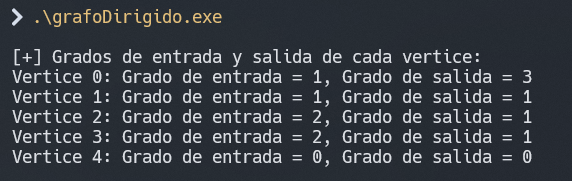
\includegraphics[width=0.7\textwidth,keepaspectratio]{img/exercise1.png}
            \end{figure}

        \subsubsection*{\texttt{GRAPHindeg}: Grado de entrada}
            Esta función calcula el número de arcos que llegan a un vértice dado \( v \). El procedimiento es el siguiente:
            \begin{enumerate}
                \item Inicializa un contador: \texttt{int indeg = 0}.
                \item Itera sobre todos los vértices del grafo (\( u \)).
                \item Para cada vértice \( u \), recorre su lista de adyacencia (\texttt{G->adj[u]}).
                \item Comprueba si \( v \) es el destino (\texttt{a->w == v}) de algún arco saliente desde \( u \).
                \item Si lo es, incrementa el contador \texttt{indeg}.
                \item Devuelve el valor acumulado del contador, que representa el grado de entrada de \( v \).
            \end{enumerate}
            
            \textbf{Complejidad:} \( O(V + A) \), donde \( V \) es el número de vértices y \( A \) es el número de arcos, porque se recorren todas las listas de adyacencia.
        
        \subsubsection*{\texttt{GRAPHoutdeg}: Grado de salida}
            Esta función calcula el número de arcos que salen de un vértice dado \( v \). El procedimiento es:
            \begin{enumerate}
                \item Inicializa un contador: \texttt{int outdeg = 0}.
                \item Recorre directamente la lista de adyacencia de \( v \) (\texttt{G->adj[v]}).
                \item Incrementa el contador por cada arco encontrado.
                \item Devuelve el valor acumulado del contador, que representa el grado de salida de \( v \).
            \end{enumerate}
            
            \textbf{Complejidad:} \( O(\deg^+(v)) \), donde \( \deg^+(v) \) es el grado de salida de \( v \), porque solo recorre la lista de adyacencia de \( v \).


    \subsection{Consideremos el problema de decidir si dos vértices son adyacentes en un grafo G. ¿Cuánto tiempo se tarda en resolver problema? Da tu respuesta en función del número de vértices y arcos del grafo.}

        \lstinputlisting[language=C++, caption={exercise2.cpp}, numbers=left]{src/exercises/exercise2.cpp}

        \textbf{Ejecución del código}
            \begin{figure}[H]
            	\centering
             	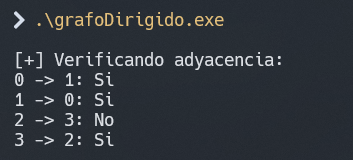
\includegraphics[width=0.7\textwidth,keepaspectratio]{img/exercise2.png}
            \end{figure}

        \subsubsection*{Descripción de la función}
            \begin{enumerate}
                \item La función recibe como parámetros:
                \begin{itemize}
                    \item Un puntero al grafo \( G \) (representado mediante listas de adyacencia).
                    \item Dos vértices \( v \) y \( w \).
                \end{itemize}
                \item Recorre la lista de adyacencia del vértice \( v \) (\texttt{G->adj[v]}).
                \item Para cada nodo en la lista, comprueba si el destino del arco (\texttt{a->w}) coincide con \( w \).
                \item Si encuentra una coincidencia, devuelve \texttt{true} (indicando que \( v \to w \) es un arco existente).
                \item Si recorre toda la lista sin encontrar \( w \), devuelve \texttt{false}.
            \end{enumerate}
            
        \subsubsection*{Complejidad de la función}
            La complejidad depende del número de arcos salientes del vértice \( v \) (es decir, su grado de salida, \( \deg^+(v) \)):
            \[
            O(\deg^+(v))
            \]
            En el peor caso, si \( v \) tiene muchos arcos, la función deberá recorrer toda su lista de adyacencia.
       

    \subsection{Escribe una función GRAPHdestroy() que destruya la representación de un grafo G, liberando el espacio que la representación ocupa en memoria.}

        \lstinputlisting[language=C++, caption={exercise3.cpp}, numbers=left]{src/exercises/exercise3.cpp}

        \subsubsection*{Descripción de la función}
            El objetivo de la función es destruir el grafo \( G \) y liberar toda la memoria asignada. El procedimiento es el siguiente:
            \begin{enumerate}
                \item Recorre todos los vértices del grafo (\( v \) de \( 0 \) a \( G->V - 1 \)).
                \item Para cada vértice \( v \):
                \begin{itemize}
                    \item Obtiene el puntero a la cabeza de su lista de adyacencia (\texttt{node *a = G->adj[v]}).
                    \item Recorre la lista de adyacencia y, para cada nodo:
                    \begin{itemize}
                        \item Almacena un puntero temporal (\texttt{temp}) al nodo actual.
                        \item Avanza al siguiente nodo de la lista (\texttt{a = a->next}).
                        \item Libera la memoria del nodo actual utilizando \texttt{delete temp}.
                    \end{itemize}
                \end{itemize}
                \item Libera el vector de listas de adyacencia (\texttt{delete[] G->adj}).
                \item Finalmente, libera la memoria asignada al propio grafo (\texttt{delete G}).
            \end{enumerate}
            
        \subsubsection*{Complejidad de la función}
            La complejidad de la función depende del número total de nodos en las listas de adyacencia. Si \( A \) es el número de arcos del grafo:
            \[
            O(V + A)
            \]
            \begin{itemize}
                \item \( O(V) \): para iterar sobre todos los vértices.
                \item \( O(A) \): para recorrer y liberar todos los nodos en las listas de adyacencia.
            \end{itemize}
            

    \subsection{Escribe una función GRAPHshow() que imprima todos los vértices adyacentes a v en una línea para cada vértice v del grafo G.}

        \lstinputlisting[language=C++, caption={exercise4.cpp}, numbers=left]{src/exercises/exercise4.cpp}

        \textbf{Ejecución del código}
            \begin{figure}[H]
            	\centering
             	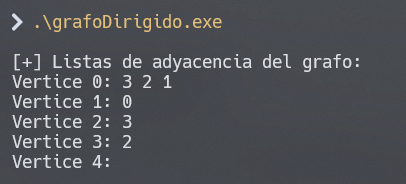
\includegraphics[width=0.7\textwidth,keepaspectratio]{img/exercise4.png}
            \end{figure}

        \subsubsection*{Descripción de la función}
            El objetivo de la función es imprimir en consola las listas de adyacencia del grafo \( G \). El procedimiento es el siguiente:
            \begin{enumerate}
                \item Recorre todos los vértices del grafo (\( v \) de \( 0 \) a \( G\rightarrow V - 1 \)).
                \item Para cada vértice \( v \):
                \begin{itemize}
                    \item Imprime el número del vértice (\texttt{\(cout << "Vertice " << v << ":"\)}).
                    \item Recorre su lista de adyacencia (\texttt{G->adj[v]}).
                    \item Para cada nodo en la lista, imprime el destino del arco almacenado en el nodo (\texttt{a->w}).
                \end{itemize}
                \item Después de imprimir todos los nodos adyacentes a \( v \), pasa a la siguiente línea.
            \end{enumerate}
            
        \subsubsection*{Complejidad de la función}
            La complejidad depende del número total de nodos en las listas de adyacencia. Si \( A \) es el número de arcos del grafo:
            \[
            O(V + A)
            \]
            \begin{itemize}
                \item \( O(V) \): para iterar sobre todos los vértices.
                \item \( O(A) \): para recorrer todas las listas de adyacencia.
            \end{itemize}


    \subsection{Eliminación de arcos. Escriba una función GRAPHremoveArc() que tome dos vértices v y w de un grafo G representado por listas de adyacencia y elimine el arco v-w de G.}

        \lstinputlisting[language=C++, caption={exercise5.cpp}, numbers=left]{src/exercises/exercise5.cpp}

        \textbf{Ejecución del código}
            \begin{figure}[H]
            	\centering
             	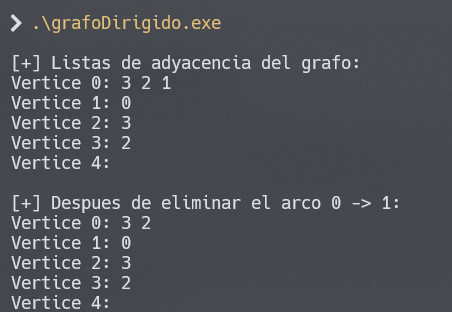
\includegraphics[width=0.7\textwidth,keepaspectratio]{img/exercise5.png}
            \end{figure}

        \subsubsection*{Descripción de la función}
            La función \texttt{GRAPHremoveArc} elimina un arco dirigido \( v \to w \) del grafo \( G \), representado mediante listas de adyacencia. El procedimiento es el siguiente:
            \begin{enumerate}
                \item Se inicializa un puntero \texttt{current} que recorre la lista de adyacencia de \( v \) (\texttt{G->adj[v]}), y un puntero \texttt{prev} para mantener el nodo previo durante la iteración.
                \item Se itera por los nodos de la lista:
                \begin{itemize}
                    \item Si se encuentra un nodo que contiene el destino \( w \) (\texttt{current->w == w}), se actualizan los punteros para desvincular dicho nodo:
                    \begin{itemize}
                        \item Si el nodo a eliminar es el primero en la lista, se ajusta la cabeza de la lista (\texttt{G->adj[v]}).
                        \item En caso contrario, el puntero \texttt{prev->next} se enlaza al nodo siguiente.
                    \end{itemize}
                    \item Se elimina el nodo encontrado utilizando \texttt{delete}.
                    \item Se decrementa el contador de arcos del grafo (\texttt{G->A}) y se termina la función con \texttt{return}.
                \end{itemize}
                \item Si se recorre toda la lista sin encontrar \( w \), no se realiza ninguna modificación.
            \end{enumerate}
            
        \subsubsection*{Complejidad de la función}
            La complejidad de la función depende de la longitud de la lista de adyacencia del vértice \( v \), lo cual equivale al grado de salida de \( v \), denotado como \( \deg^+(v) \):
            \[
            O(\deg^+(v))
            \]
            
            En el peor caso:
            \begin{itemize}
                \item Si \( w \) no se encuentra en la lista de adyacencia, se recorrerá toda la lista.
                \item Si \( v \) tiene muchos arcos salientes (\( \deg^+(v) \) es grande), el tiempo será proporcional a la cantidad de arcos salientes.
            \end{itemize}
            

    \subsection{¿No dirigido? Escriba una función GRAPHundir() que decida si un grafo dado es no dirigido.}

        \lstinputlisting[language=C++, caption={exercise6.cpp}, numbers=left]{src/exercises/exercise6.cpp}

        \textbf{Ejecución del código}
            \begin{figure}[H]
            	\centering
             	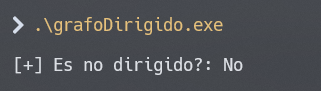
\includegraphics[width=0.7\textwidth,keepaspectratio]{img/exercise6.png}
            \end{figure}

        \subsubsection*{Descripción de la función}
            La función \texttt{GRAPHundir} verifica si un grafo dirigido \( G \), representado mediante listas de adyacencia, es no dirigido. Un grafo es considerado no dirigido si, para cada arco \( v \to w \), también existe el arco \( w \to v \).
            
            El procedimiento es el siguiente:
            \begin{enumerate}
                \item Se recorre cada vértice \( v \) del grafo (\texttt{for (int v = 0; v < G->V; ++v)}).
                \item Para cada vértice \( v \), se itera sobre los nodos en su lista de adyacencia (\texttt{G->adj[v]}), obteniendo cada destino \( w \) (\texttt{a->w}).
                \item Para cada arco \( v \to w \), se recorre la lista de adyacencia de \( w \) para buscar un arco \( w \to v \).
                \item Si no se encuentra \( w \to v \), la función devuelve \texttt{false}, indicando que el grafo no es no dirigido.
                \item Si se verifican todos los vértices y arcos sin encontrar inconsistencias, la función devuelve \texttt{true}.
            \end{enumerate}
            
        \subsubsection*{Complejidad de la función}
            La complejidad depende del número de vértices \( V \) y arcos \( A \). Para cada arco \( v \to w \), se busca su correspondiente arco \( w \to v \) recorriendo la lista de adyacencia de \( w \). Esto lleva a una complejidad:
            \[
            O(A \cdot \Delta)
            \]
            donde \( \Delta \) es el grado máximo del grafo (la longitud máxima de una lista de adyacencia).


    \subsection{Inserción de aristas. Escribe una función UGRAPHinsertEdge() que inserte una arista v-w en un grafo no dirigido G.}

        \lstinputlisting[language=C++, caption={exercise7.cpp}, numbers=left]{src/exercises/exercise7.cpp}

        \textbf{Ejecución del código}
            \begin{figure}[H]
            	\centering
             	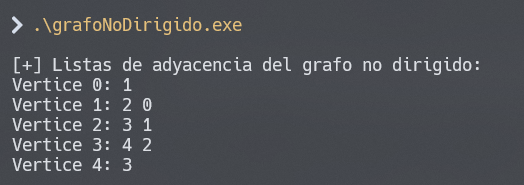
\includegraphics[width=0.7\textwidth,keepaspectratio]{img/exercise7.png}
            \end{figure}

        \subsubsection*{Descripción de la función}
            La función \texttt{UGRAPHinsertEdge} inserta una arista no dirigida \( v-w \) en un grafo representado mediante listas de adyacencia. Para lograrlo:
            \begin{enumerate}
                \item Verifica si el arco \( v \to w \) ya existe en la lista de adyacencia de \( v \). Si no, lo agrega y actualiza el contador de arcos.
                \item Verifica si el arco \( w \to v \) ya existe en la lista de adyacencia de \( w \). Si no, lo agrega y también incrementa el contador.
            \end{enumerate}
            De esta forma, asegura que ambos extremos de la arista estén representados.
            
        \subsubsection*{Complejidad de la función}
            La complejidad es proporcional a las longitudes de las listas de adyacencia de \( v \) y \( w \):
            \[
            O(\deg^+(v) + \deg^+(w))
            \]
            Esto la hace eficiente para grafos dispersos, pero más costosa en grafos densos con listas de adyacencia largas.


    \subsection{Eliminación de aristas. Escribe una función UGRAPHremoveEdge() que elimine una arista dada v-w de un grafo no dirigido G.}

        \lstinputlisting[language=C++, caption={exercise8.cpp}, numbers=left]{src/exercises/exercise8.cpp}

        \textbf{Ejecución del código}
            \begin{figure}[H]
            	\centering
             	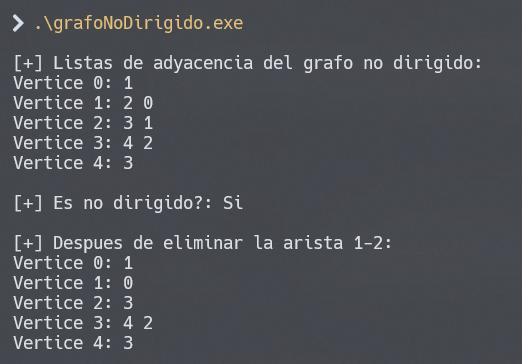
\includegraphics[width=0.7\textwidth,keepaspectratio]{img/exercise8.png}
            \end{figure}

        \subsubsection*{Descripción de la función}
            La función \texttt{UGRAPHremoveEdge} elimina una arista no dirigida \( v-w \) de un grafo representado mediante listas de adyacencia. Esto implica:
            \begin{enumerate}
                \item Recorrer la lista de adyacencia de \( v \) para eliminar el arco \( v \to w \).
                \item Recorrer la lista de adyacencia de \( w \) para eliminar el arco \( w \to v \).
                \item En ambos casos, actualiza los punteros de la lista para desvincular el nodo correspondiente y libera su memoria.
                \item Decrementa el contador de arcos (\texttt{G->A}) por cada arco eliminado.
            \end{enumerate}
            De esta forma, se garantiza que la arista no dirigida \( v-w \) sea completamente eliminada.
            
        \subsubsection*{Complejidad de la función}
            La complejidad es proporcional a las longitudes de las listas de adyacencia de \( v \) y \( w \), ya que estas deben recorrerse para encontrar y eliminar los nodos correspondientes:
            \[
            O(\deg^+(v) + \deg^+(w))
            \]
            Esto la hace eficiente para grafos dispersos, pero menos eficiente en grafos densos donde las listas de adyacencia son largas.

\section{Código main final}
    \subsection{Código main final del grafo dirigido}
        \lstinputlisting[language=C++, caption={mainDirigido.cpp}, numbers=left]{src/exercises/mainDirigido.cpp}

    \subsection{Código main final del grafo NO dirigido}
        \lstinputlisting[language=C++, caption={mainNoDirigido.cpp}, numbers=left]{src/exercises/mainNoDirigido.cpp}

            
%%% REPOSITORIO DE GITHUB %%%
\section{Repositorio de Github}
	\begin{itemize}
		\item Repositorio de Github donde se encuentra el actual laboratorio \\
		\url{https://github.com/ReyserLynnn/ada-lab-b-24b/tree/main/laboratorio06/src}

        \item Repositorio de Github donde se encuentran los laboratorios del curso\\
		\url{https://github.com/ReyserLynnn/ada-lab-b-24b.git}
	\end{itemize}

\section{Conclusión}
	para finalizar el informe, entendí cómo manipular grafos usando listas de adyacencia, desde agregar y eliminar conexiones hasta verificar y mostrar su estructura. Analizar su complejidad y su utilidad práctica en diferentes tipos de grafos es de ayuda para comprender al 100\%.

\begin{comment}
\section{Referencias}
\begin{itemize}			
	\item \url{https://dialnet.unirioja.es/servlet/articulo?codigo=4573315}
\end{itemize}	    
\end{comment}

\end{document}